\section{Příklad 4}
% Jako parametr zadejte skupinu (A-H)
\ctvrtyZadani{H}

\subsection{Vypocet jednotlivych impedancii}

Najskor si musime vypocitat impedancie zavisle na uhlovej frekvencii pre kondenzatory a cievky.

\begin{align*}
    \omega &= 2\pi f = 2 \pi \cdot 95 = 596.902604182\\
    Z_{C1} &= \frac{-j}{\omega C} = \frac{-j}{596.902604182 \cdot \SI{155}{\micro\farad}} = \SI{-10.8084850j}{\ohm}\\
    Z_{C2} &= \frac{-j}{\omega C} = \frac{-j}{596.902604182 \cdot \SI{70}{\micro\farad}} = \SI{-23.9330741j}{\ohm}\\
    Z_{L1} &= j\omega L = j \cdot 596.902604182 \cdot \SI{160}{\micro\henry} = \SI{95.5044166j}{\ohm}\\
    Z_{L2} &= j\omega L = j \cdot 596.902604182 \cdot \SI{75}{\micro\henry} = \SI{44.7676953j}{\ohm}\\
\end{align*}

\subsection{Zostrojenie matice}

\begin{figure}[!h]
    \centering
    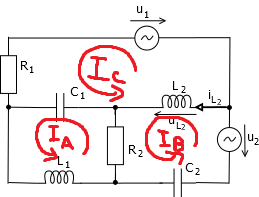
\includegraphics[width=0.5\linewidth]{pr4/1.png}
\end{figure}

Aby sme mohli pouzit metodu smyckovych prudov, musime si najskor vytvorit maticu. 
Tato matica bude mat na hlavnej diagonale sucet impedancii vsetkych prvkov v danej smycke.
Na ostatnych poziciach potom budu zaporne zobrate prvky, ktore maju dane dve smycky spolocne.
\newpage

\begin{figure}[!h]
    \centering
    \begin{equation}
    \begin{pmatrix}
    R_2 + Z_{C1} + Z_{L1} & -R_2 & -Z_{C1}\\
    -R_2  & R_2 + Z_{C2} + Z_{L2} & -Z_{L2}\\
    -Z_{C1} & -Z_{L2} & R_1 + Z_{C1} + Z_{L2} \\
    \end{pmatrix}
    \cdot
    \begin{pmatrix}
    I_A\\
    I_B\\
    I_C\\
    \end{pmatrix}
    =
    \begin{pmatrix}
    0\\
    U_2\\
    U_1\\
    \end{pmatrix}
    \end{equation}
\end{figure}

\begin{figure}[!h]
    \centering
    \begin{equation}
    \begin{pmatrix}
    \SI{10 + 84.6959316j}{\ohm}&\SI{-10}{\ohm}&\SI{10.8084850j}{\ohm}\\
    \SI{-10}{\ohm}&\SI{10 + 20.8346212j}{\ohm}&\SI{-44.7676953j}{\ohm}\\\
    \SI{10.8084850j}{\ohm}&\SI{-44.7676953j}{\ohm}&\SI{10 + 33.9592103j}{\ohm}\\
    \end{pmatrix}
    \cdot
    \begin{pmatrix}
    I_A\\
    I_B\\
    I_C\\
    \end{pmatrix}
    =
    \begin{pmatrix}
    0\\
    60V\\
    65V\\
    \end{pmatrix}
    \end{equation}
\end{figure}

\begin{align*}
    I_A &=  \SI{0.1858119-0.4679328j}{\ampere}\\
    I_B &= \SI{1.691498+2.728377j}{\ampere}\\
    I_C &= \SI{1.501190+2.273690j}{\ampere}\\
\end{align*}

\subsection{Vypocet $|U_{L2}|$ a $\varphi_{L2}$}
\begin{align*}
    i_{L2} &= I_B - I_C = \SI{1.691498+2.728377j}{\ampere} - \SI{1.501190+2.273690j}{\ampere} = \SI{0.190308 + 0.454687j}{\ampere}\\
    u_{L2} &= i_{L2} \cdot Z_{L2} = \SI{3.192688 + 5.002067j}{\ampere} \cdot \SI{44.7676953j}{\ohm} = \SI{-20.3552891 + 8.5196506i}{\volt}\\
    |U_{L2}| &= \sqrt{u \cdot u} = \SI{22.06631461}{\volt}\\
    \varphi_{L2} &= \arctan \frac{Imaginary(u_{L2})}{Real(u_{L2})} = -22.7116146 \degree
\end{align*}